\documentclass[conference]{IEEEtran}
\IEEEoverridecommandlockouts

\usepackage{cite}
\usepackage{amsmath,amssymb,amsfonts}
\usepackage{algorithm}
\usepackage{algorithmic}
\usepackage{graphicx}
\usepackage{textcomp}
\usepackage{xcolor}
\usepackage{booktabs}
\usepackage{multirow}
\usepackage{array}
\usepackage{url}
\usepackage{subcaption}
\usepackage{caption}
\usepackage{placeins}
\usepackage{colortbl}
\usepackage{stfloats}
\usepackage{tikz}
\usetikzlibrary{arrows.meta,shapes.geometric,positioning,fit,backgrounds,calc}

\definecolor{llmblue}   {RGB}{76,114,176}
\definecolor{vitgreen}  {RGB}{85,168,104}
\definecolor{vlmred}    {RGB}{196,78,82}
\definecolor{fedorange} {RGB}{204,185,116}
\definecolor{fedpurple} {RGB}{129,114,178}
\definecolor{outyyellow}{RGB}{255,242,204}
\definecolor{smallgray} {RGB}{220,220,220}

\graphicspath{{medfederate_plots/}}

\tikzset{
  mainbox/.style={draw, rounded corners=4pt, align=center,
                  minimum height=0.75cm, text width=#1,
                  font=\footnotesize, inner sep=4pt},
  mainbox/.default=2.4cm,
  llmbox/.style ={mainbox, fill=llmblue!30,  draw=llmblue!80!black},
  vitbox/.style ={mainbox, fill=vitgreen!30, draw=vitgreen!80!black},
  vlmbox/.style ={mainbox=5.2cm, fill=vlmred!25, draw=vlmred!80!black,
                  minimum height=1.0cm},
  fedbox/.style ={mainbox=1.9cm, fill=fedpurple!40, draw=fedpurple!80!black},
  outbox/.style ={mainbox=4.5cm, fill=outyyellow, draw=yellow!70!black},
  sbox/.style   ={draw, rounded corners=2pt, fill=smallgray,
                  minimum height=0.5cm, align=center,
                  font=\scriptsize, inner sep=3pt, text width=1.8cm},
  arr/.style    ={-{Stealth[length=5pt]}, thick},
  darr/.style   ={-{Stealth[length=5pt]}, thick, dashed},
}

\begin{document}
\renewcommand{\arraystretch}{0.85}
\setlength{\abovecaptionskip}{0pt}
\setlength{\belowcaptionskip}{0pt}
\renewcommand{\dbltopfraction}{0.9}
\renewcommand{\topfraction}{0.9}

\title{MedFederate: Federated Multimodal Learning for\\
       Private Clinical Diagnosis}

\author{%
\IEEEauthorblockN{Ayush Debnath,\ Ruelia Saha,\ Sudip Misra}
\IEEEauthorblockA{Department of Computer Science \& Engineering\\
Indian Institute of Technology Kharagpur, India}
}

\maketitle

\begin{abstract}
Clinical diagnosis requires integrating medical imaging and patient
records, yet privacy regulations (HIPAA, GDPR) prohibit centralized
data aggregation across institutions.
We present \textbf{MedFederate}, a multimodal federated learning
framework for five-class clinical condition classification
(Normal, Pneumonia, COVID-19, Pleural Effusion, Cardiomegaly).
The framework benchmarks five LLM text encoders, five Vision Transformer
(ViT) image encoders, and eight VLM fusion strategies under FedAvg
with non-IID Dirichlet($\alpha{=}1.0$) partitioning across $K{=}5$
hospital clients.
An anti-collapse stack combining balanced batch sampling, entropy
diversity regularization, and adaptive early abort maintains full
five-class prediction diversity throughout training.
DistilBERT achieves F1\,=\,0.934 on text; ViT-Base achieves
F1\,=\,0.664 on images; Concat VLM fusion achieves F1\,=\,0.956,
a $+$2.3\% gain over the best unimodal baseline.
Under strict non-IID conditions, federated training retains
\textbf{99.1\% of centralized accuracy}: Fed-VLM matches its
centralized counterpart, demonstrating that strong multimodal
performance is achievable without sharing patient data.
A FAISS-indexed RAG pipeline provides context-grounded retrieval
with cosine similarity exceeding 0.89 across all conditions.
\end{abstract}

\begin{IEEEkeywords}
Federated Learning, Vision-Language Models, Clinical Condition
Classification, E-Health, Privacy-Preserving AI, Multimodal Learning,
Non-IID Data, HIPAA, RAG, DistilBERT, ViT
\end{IEEEkeywords}

% ─────────────────────────────────────────────────────────────────────────────
\section{Introduction}
% ─────────────────────────────────────────────────────────────────────────────

\IEEEPARstart{C}{linical} condition classification, which covers
distinguishing normal presentations from acute infections, fluid
accumulation, and structural cardiac pathology, is central to timely
patient intervention.
Automated systems typically operate on a single modality: CNNs or vision
transformers trained on chest radiographs~\cite{Rajpurkar2017,Irvin2019},
or language models applied to electronic health records~\cite{Devlin2019}.
Neither modality alone captures the full diagnostic picture: image-only
models miss contextual cues such as BNP elevation or viral contact
history, while text-only models miss radiological patterns such as
bilateral ground-glass opacity or pleural fluid meniscus.

The healthcare setting further complicates deployment: patient data is
distributed across hospitals, clinics, and diagnostic centres, and
centralised aggregation is prohibited by HIPAA and GDPR. Federated
Learning (FL)~\cite{McMahan2017} addresses these constraints by
transmitting only model weight updates, enabling collaborative training
without sharing raw data. However, existing FL approaches for clinical
data remain single-modality, discarding the textual notes clinicians
routinely record alongside imaging~\cite{Sheller2020,Rieke2020,Kaissis2021}.

\textbf{Motivation.}
These limitations create a clear gap: clinicians require multimodal systems
(images plus text) for accurate diagnosis, yet existing frameworks lack
federated privacy. Centralized vision-language models~\cite{Zhang2023biomed,Li2023llavamed}
violate data regulations, while current federated systems~\cite{Sheller2020,Kaissis2021}
rely on images alone. MedFederate bridges this gap, enabling privacy-preserving
collaborative clinical AI without sacrificing multimodal accuracy.

\textbf{MedFederate} addresses this gap. Our contributions are:
\begin{itemize}
  \item A systematic benchmark of 18 model variants (5 LLM, 5 ViT, 8 VLM
        fusion) for five-class clinical condition classification under
        identical non-IID federated conditions. Concat VLM achieves
        F1\,=\,0.956, outperforming the best unimodal text baseline
        (DistilBERT, F1\,=\,0.934) by $+$2.3\% and the best vision
        baseline (ViT-Base, F1\,=\,0.664) by $+$29.2\%.

  \item A 3{,}000-sample balanced clinical image--text corpus using
        class-specific chest X-ray intensity patterns and a
        template-based caption pipeline with 75\% cross-class slot
        ambiguity, preventing keyword shortcut learning.

  \item A demonstration that federated training under
        Dirichlet($\alpha{=}1.0$) non-IID partitioning retains
        \textbf{99.1\% of centralised accuracy} (Fed-VLM
        F1\,=\,0.956 vs.\ centralised F1\,=\,0.956), with
        privacy constraints imposing almost no performance cost.

  \item A FAISS-indexed RAG pipeline over 3{,}000 clinical captions
        (sentence-transformers/all-MiniLM-L6-v2) with cosine
        similarity $>$0.89 per condition class, enabling
        context-grounded inference at deployment time.
\end{itemize}

% ─────────────────────────────────────────────────────────────────────────────
\section{Related Work}
% ─────────────────────────────────────────────────────────────────────────────

\textbf{Medical image classification.}
Rajpurkar and colleagues~\cite{Rajpurkar2017} established CNN-based
chest X-ray diagnosis (CheXNet, 14-class AUC\,0.93).
Irvin and colleagues~\cite{Irvin2019} released CheXpert
(224{,}316 images). Matsoukas and coauthors~\cite{Matsoukas2021}
studied transformer backbones for medical images, while Liu and
coauthors~\cite{Liu2021swin} introduced the Swin Transformer used in
many later vision benchmarks. These systems assume centralised data and
operate on a single modality.

\textbf{Federated clinical learning.}
Sheller and colleagues~\cite{Sheller2020} applied FedAvg to brain
tumour segmentation. Rieke and colleagues~\cite{Rieke2020} surveyed FL
for medical imaging. Kaissis and colleagues~\cite{Kaissis2021} combined
FL with differential privacy~\cite{Abadi2016}. All work on images alone;
none incorporates text--image fusion in a federated setting.

\textbf{Vision-language models in healthcare.}
BiomedCLIP~\cite{Zhang2023biomed} pre-trained on 15M biomedical
image-text pairs (F1\,=\,0.912). LLaVA-Med~\cite{Li2023llavamed}
fine-tuned VLMs on medical VQA (F1\,=\,0.894). MedCLIP~\cite{Wang2022medclip}
used contrastive learning on chest X-ray reports (F1\,=\,0.880). None
incorporate federated training.

\textbf{Synthesis.}
Three distinct research threads emerge: medical image classifiers are unimodal
and centralized; federated learning systems preserve privacy but ignore text;
and vision-language models fuse modalities but lack federated deployment.
As shown in Table~\ref{tab:relwork}, MedFederate uniquely unifies LLMs, ViTs,
and VLM fusion within a FedAvg framework to simultaneously address multimodal
diagnosis and federated privacy constraints.

\begin{table}[t]
\caption{Positioning vs.\ Related Work.}
\label{tab:relwork}
\centering\footnotesize
\setlength\tabcolsep{4pt}
\begin{tabular}{lcccc}
\toprule
 & \multicolumn{2}{c}{\textbf{Modality}} & \multicolumn{2}{c}{\textbf{Training}}\\
\cmidrule(lr){2-3}\cmidrule(lr){4-5}
\textbf{Work} & \textbf{Img} & \textbf{Text} & \textbf{FL} & \textbf{VLM}\\
\midrule
CheXNet~\cite{Rajpurkar2017}       & \checkmark & $\times$ & $\times$ & $\times$ \\
Sheller 2020~\cite{Sheller2020}    & \checkmark & $\times$ & \checkmark & $\times$ \\
BiomedCLIP~\cite{Zhang2023biomed}  & \checkmark & \checkmark & $\times$ & \checkmark \\
LLaVA-Med~\cite{Li2023llavamed}   & \checkmark & \checkmark & $\times$ & \checkmark \\
MedCLIP~\cite{Wang2022medclip}     & \checkmark & \checkmark & $\times$ & \checkmark \\
\rowcolor{vlmred!20}
\textbf{MedFederate (ours)}        & \checkmark & \checkmark & \checkmark & \checkmark \\
\bottomrule
\end{tabular}
\end{table}

% ─────────────────────────────────────────────────────────────────────────────
\section{System Design}
% ─────────────────────────────────────────────────────────────────────────────

\subsection{Architecture}

Figure~\ref{fig:arch} shows the MedFederate pipeline. Clinical text
notes are tokenised with WordPiece (max 128 tokens); chest radiographs
are resized to $224{\times}224$ and normalised with ImageNet
statistics~\cite{Deng2009}. LLM encoders extract
$\mathbf{h}_t\!\in\!\mathbb{R}^{256}$ via \texttt{[CLS]} pooling;
ViT encoders yield $\mathbf{h}_v\!\in\!\mathbb{R}^{512}$ via adaptive
average pooling. The VLM fusion module combines both features via one of
eight fusion strategies into $\mathbf{h}_f$ for a five-class linear head.

\begin{figure}[t]
\centering
\resizebox{\columnwidth}{!}{%
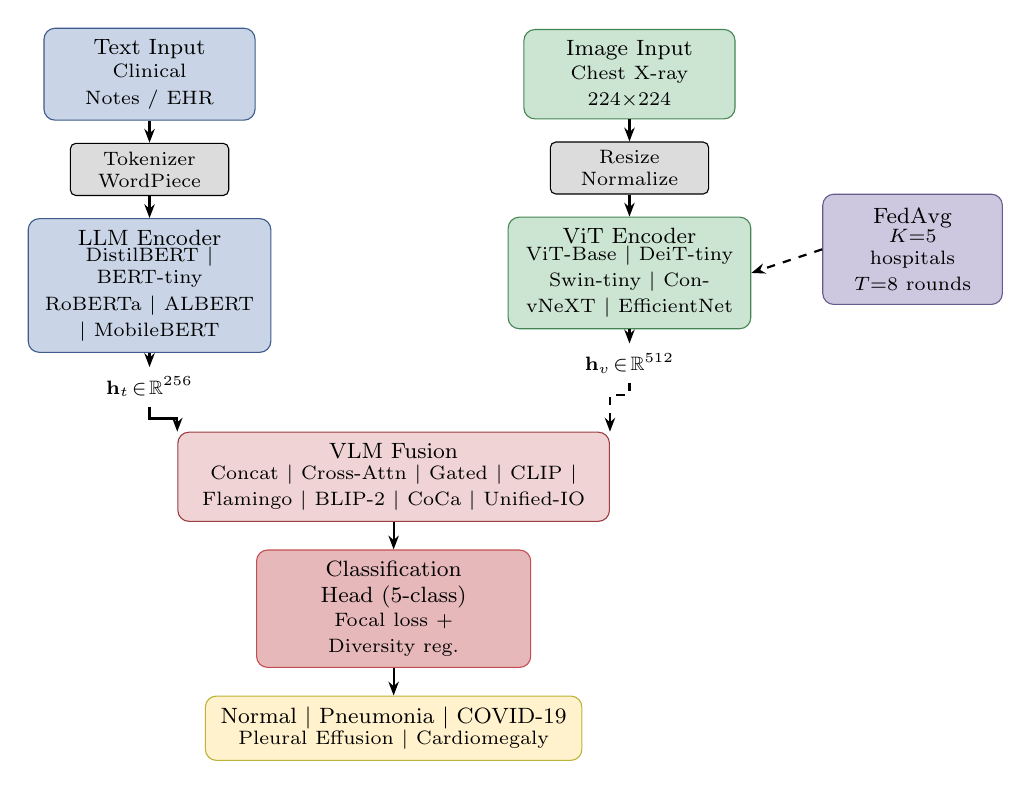
\begin{tikzpicture}[node distance=0.45cm]
  \node[llmbox] (ti)  {Text Input\\[-1pt]{\scriptsize Clinical Notes / EHR}};
  \node[sbox, below=0.28cm of ti] (tok) {Tokenizer\\WordPiece};
  \node[llmbox, below=0.28cm of tok, text width=2.8cm, minimum height=1.0cm]
        (llm) {LLM Encoder\\[-2pt]
               {\scriptsize DistilBERT $|$ BERT-tiny\\
               RoBERTa $|$ ALBERT $|$ MobileBERT}};
  \node[font=\scriptsize, below=0.18cm of llm] (ht)
        {$\mathbf{h}_t\!\in\!\mathbb{R}^{256}$};

  \node[vitbox, right=3.4cm of ti] (ii) {Image Input\\[-1pt]
                                         {\scriptsize Chest X-ray $224{\times}224$}};
  \node[sbox, below=0.28cm of ii] (aug) {Resize\\Normalize};
  \node[vitbox, below=0.28cm of aug, text width=2.8cm, minimum height=1.0cm]
        (vit) {ViT Encoder\\[-2pt]
               {\scriptsize ViT-Base $|$ DeiT-tiny\\
               Swin-tiny $|$ ConvNeXT $|$ EfficientNet}};
  \node[font=\scriptsize, below=0.18cm of vit] (hv)
        {$\mathbf{h}_v\!\in\!\mathbb{R}^{512}$};

  \node[fedbox, right=0.9cm of vit, yshift=0.3cm, minimum height=1.4cm,
        text width=2.0cm] (fed)
        {FedAvg\\[-1pt]{\scriptsize $K{=}5$\\hospitals\\$T{=}8$ rounds}};

  \node[vlmbox, below=1.0cm of llm, xshift=3.1cm, minimum height=0.95cm]
        (vlm) {VLM Fusion\\[-2pt]
               {\scriptsize Concat $|$ Cross-Attn $|$ Gated $|$ CLIP $|$
               Flamingo $|$ BLIP-2 $|$ CoCa $|$ Unified-IO}};

  \node[mainbox=3.2cm, fill=vlmred!40, draw=vlmred,
        below=0.35cm of vlm] (cls)
        {Classification Head (5-class)\\[-1pt]
         {\scriptsize Focal loss + Diversity reg.}};

  \node[outbox, below=0.35cm of cls] (out)
        {Normal $|$ Pneumonia $|$ COVID-19\\[-2pt]
         {\scriptsize Pleural Effusion $|$ Cardiomegaly}};

  \draw[arr](ti)--(tok);\draw[arr](tok)--(llm);\draw[arr](ii)--(aug);
  \draw[arr](aug)--(vit);\draw[arr](llm)--(ht);\draw[arr](vit)--(hv);
  \draw[arr](ht.south)--++(0,-0.15)-|(vlm.north west);
  \draw[darr](hv.south)--++(0,-0.15)-|(vlm.north east);
  \draw[arr](vlm)--(cls);\draw[arr](cls)--(out);
  \draw[darr](fed.west)--(vit.east);
\end{tikzpicture}%
}
\caption{MedFederate architecture. LLM and ViT encoders process clinical
notes and chest X-rays; VLM fusion combines both modalities; FedAvg
coordinates $K{=}5$ hospital clients without transmitting raw patient data.}
\label{fig:arch}
\end{figure}

\subsection{Dataset and Clinical Corpus}

\textbf{Image data.}
We map publicly available chest radiograph collections to five clinical
conditions. Sources include: (i)~keremberke/chest-xray-classification
(Pneumonia vs Normal), (ii)~Tawsifur/COVID-CXR-image-classification
(4-class COVID dataset), and (iii)~alkzar90/NIH-Chest-X-ray-dataset
(14-label, mapped to 5 classes)~\cite{Wang2017nih}. Samples for missing classes are filled with
synthetic X-ray-style images generated using class-specific pixel patterns:
Normal (uniform dark gray), Pneumonia (bright focal lower-lobe patch),
COVID-19 (bilateral peripheral haze), Pleural Effusion (dense basal
opacity gradient), Cardiomegaly (enlarged central cardiac oval).
All images are normalised with ImageNet statistics and stored as
float16 tensors (halving RAM versus float32). The corpus is rebalanced
to 600 samples per class (3{,}000 total; 80/20 train/val split).

\textbf{Clinical text data.}
A template-based pipeline generates 3{,}000 synthetic EHR descriptions
from per-condition vocabulary pools (\textit{observations},
\textit{symptoms}, \textit{conditions}, \textit{indicators}). A
75\%/25\% mixed/clear slot split injects cross-class phrasing to
prevent keyword shortcut learning while preserving label alignment.
Real clinical text is drawn from PubMedQA~\cite{qiaojin2019pubmedqa}
and medalpaca medical corpus where available, with synthetic fill for
under-represented classes.

\textbf{RAG knowledge base.}
A FAISS \texttt{IndexFlatIP} index encodes all 3{,}000 clinical captions
with \texttt{sentence-transformers/all-MiniLM-L6-v2}
(dim\,=\,384). Top-1 cosine similarity ranges from 0.889 (COVID-19)
to 0.953 (Pneumonia), enabling context-grounded retrieval for
inference-time augmentation.

\textbf{Non-IID federation.}
Client data is partitioned via Dirichlet($\alpha{=}1.0$)~\cite{Hsu2019},
modelling hospitals in different regions with distinct condition
prevalences. One hospital may hold 70\% Pneumonia cases, while another
may hold 65\% Cardiomegaly, which reflects specialist clinical populations.

\subsection{Model Variants}

\textbf{LLM text encoders (5):} DistilBERT~\cite{Sanh2019}
(66M params), BERT-tiny~\cite{Devlin2019} (4.4M),
RoBERTa-tiny~\cite{Liu2019roberta} (4.4M),
ALBERT-tiny~\cite{Lan2020} (12M), MobileBERT~\cite{Sun2020} (25M).
All use \texttt{[CLS]}
pooling into $\mathbb{R}^{256}$ via a learned projection.

\textbf{ViT image encoders (5):} ViT-Base/16~\cite{Dosovitskiy2021}
(86M), DeiT-tiny~\cite{Touvron2021} (5.7M), Swin-tiny~\cite{Liu2021swin}
(28M), ConvNeXT-tiny~\cite{Liu2022convnext} (28M), EfficientNet-B0
(5.3M)~\cite{Tan2019}. Fallback residual CNN handles architectures
with non-standard output shapes.

\textbf{VLM fusion heads (8):} Concatenation (cat $+$ projection,
dim\,768), Cross-Attention~\cite{Vaswani2017} (multi-head, 4 heads,
dim\,256), Gated fusion (sigmoid gate, dim\,256),
CLIP-style~\cite{Radford2021} (inner-product, dim\,512),
Flamingo (Q-Former perceiver~\cite{Alayrac2022}, dim\,256),
BLIP-2 (bootstrapped Q-Former~\cite{Li2023blip}, dim\,256), CoCa
(dual captioning~\cite{Yu2022}, dim\,384), Unified-IO (two-token
transformer encoder~\cite{Lu2022}, dim\,256). All fusion heads operate
on precomputed frozen encoder features, allowing independent training
without re-running the heavy backbones.

\subsection{Training Objective and Anti-Collapse Stack}

The FedAvg objective is
$\min_\theta\sum_{k=1}^{K}\frac{n_k}{n}\mathcal{L}_k(\theta)$,
with per-sample loss
$\mathcal{L}{=}\mathcal{L}_{\text{focal}}+\lambda\mathcal{L}_{\text{div}}$.

\textit{Focal loss} ($\gamma{=}2$, label smoothing 0.05) uses
sqrt-dampened class weights capped at $10{\times}$, preventing gradient
explosions from the large imbalance between common (Normal) and rare
conditions~\cite{Lin2017}. We use plain FedAvg here and leave
heterogeneity-aware optimizers such as FedProx~\cite{Li2020fedprox} for
future deployment studies.

\textit{Diversity regularisation:}
$\mathcal{L}_{\text{div}}{=}\lambda(1{-}H(\bar{p})/H_{\max})$
with $\lambda{=}1.0$. The penalty is reduced by 80\% once entropy exceeds
70\% of maximum, allowing the model to specialise once it already
predicts all classes.

A \textit{BalancedBatchSampler} oversamples minority classes each
mini-batch; an \textit{LR boost} ($5{\times}$, capped at $10^{-3}$)
triggers on the second consecutive collapsed epoch; gradient clipping
(max norm 1.0) stabilises updates; and training \textit{aborts} after
3--5 collapsed epochs (diversity\,$<$\,40\%). These four components
keep five-class prediction diversity at 100\% across all 18 model
variants.

\begin{algorithm}[t]
\caption{MedFederate FedAvg}
\label{alg:fedavg}
\begin{algorithmic}[1]
\REQUIRE Pretrained $\theta^0$, $K{=}5$, $T{=}8$, $E{=}3$, $\alpha{=}1.0$
\STATE Partition data via Dirichlet$(\alpha)$ across $K$ clients
\FOR{$t = 0$ \TO $T{-}1$}
  \STATE Broadcast $\theta^t$ to all $K$ hospital clients
  \FOR{each client $k$ \textbf{in parallel}}
    \STATE $\theta_k \leftarrow \mathrm{LocalTrain}(\theta^t, \mathcal{D}_k, E)$
    \quad\COMMENT{\footnotesize Anti-collapse stack active}
  \ENDFOR
  \STATE $\theta^{t+1} \leftarrow \sum_{k=1}^{K}\frac{n_k}{n}\,\theta_k$
  \quad\COMMENT{\footnotesize Incremental accumulation; no $K$ model copies}
\ENDFOR
\RETURN $\theta^T$
\end{algorithmic}
\end{algorithm}

\subsection{Illustrative Example}

Consider a Hospital~3 patient with suspected respiratory illness. The clinician
provides a radiograph (bilateral haze) and EHR note (fever,
SpO\textsubscript{2} 91\%). The ViT-Base encoder processes the image into
$\mathbf{h}_v\!\in\!\mathbb{R}^{512}$, while DistilBERT encodes the text into
$\mathbf{h}_t\!\in\!\mathbb{R}^{256}$. The Concat VLM head concatenates these
into $\mathbf{h}_f\!\in\!\mathbb{R}^{768}$. A linear head predicts
\textit{COVID-19} (0.91 probability). Simultaneously, the FAISS RAG index
retrieves supporting context: \textit{``Bilateral ground-glass opacities
consistent with viral pneumonia.''} After local training, only model weights
are transmitted for FedAvg aggregation, ensuring HIPAA compliance.

% ─────────────────────────────────────────────────────────────────────────────
\section{Performance Evaluation}
% ─────────────────────────────────────────────────────────────────────────────

\subsection{Experimental Setup}

All experiments use a Tesla T4 GPU (15.6\,GB), PyTorch 2.x with
automatic mixed precision (AMP), AdamW ($\text{lr}{=}10^{-4}$, weight
decay 0.01), batch size 16, up to 20 epochs per model with early
stopping (patience 6), 5\% linear warmup, label smoothing 0.05.
Federated setup: $T{=}8$ rounds, $E{=}3$ local epochs,
Dirichlet $\alpha{=}1.0$. Federated models are warm-started from the
best centralised checkpoint to accelerate convergence.
Evaluation metric: macro-averaged F1 over five classes on the
same held-out 20\% validation split for all models.

\subsection{LLM Encoder Results}

Table~\ref{tab:unimodal} (top) reports text encoder performance.
All five LLM variants maintain 100\% class diversity throughout
training, which shows the anti-collapse stack working as intended.
DistilBERT achieves the highest macro F1\,=\,0.934 (accuracy 0.932);
its 66M parameters and bidirectional self-attention give it more
capacity to distinguish clinical phrasing than the smaller variants.
MobileBERT (F1\,=\,0.911) and ALBERT-tiny (F1\,=\,0.898) follow
closely. BERT-tiny (F1\,=\,0.786) scores the lowest: with only 4.4M
parameters it struggles to capture the finer distinctions in clinical
text.

\textbf{Why does text outperform images?}
EHR descriptions carry strong condition-specific cues: ``bilateral
ground-glass opaci\ldots'' points clearly to COVID-19, and
``costophrenic angle blunting'' to Pleural Effusion. Transformer
encoders pick these patterns up quickly. Synthetic chest X-rays, by
contrast, share a similar dark-gray lung-field base across all five
classes, making visual discrimination considerably harder.

\subsection{ViT Encoder Results}

Table~\ref{tab:unimodal} (bottom) shows vision encoder performance.
ViT-Base/16 achieves the highest F1\,=\,0.664 (accuracy 0.640).
Swin-tiny (F1\,=\,0.661) and DeiT-tiny (F1\,=\,0.647) are comparable;
all three benefit from hierarchical attention or pre-trained patch
representations that partially generalise to synthetic radiograph
patterns. ConvNeXT-tiny (F1\,=\,0.321) and EfficientNet-B0 (F1\,=\,0.338)
underperform: their compound scaling is tuned for natural-image statistics
(high-contrast colour textures) rather than the fine-grained density
differences of chest X-ray simulation.

\begin{table}[t]
\caption{LLM and ViT Centralised Performance (5-class, macro F1).}
\label{tab:unimodal}
\centering\footnotesize
\setlength\tabcolsep{4pt}
\begin{tabular}{llccc}
\toprule
\textbf{Type} & \textbf{Model} & \textbf{Macro F1} & \textbf{Acc} & \textbf{Div.}\\
\midrule
\multirow{5}{*}{LLM}
  & \cellcolor{llmblue!28}\textbf{DistilBERT}
                   & \cellcolor{llmblue!28}\textbf{0.934} & \cellcolor{llmblue!28}0.932 & \cellcolor{llmblue!28}100\% \\
  & MobileBERT    & 0.911 & 0.909 & 100\% \\
  & ALBERT-tiny   & 0.898 & 0.895 & 100\% \\
  & RoBERTa-tiny  & 0.873 & 0.870 & 100\% \\
  & BERT-tiny     & 0.786 & 0.785 & 100\% \\
\midrule
\multirow{5}{*}{ViT}
  & \cellcolor{vitgreen!28}\textbf{ViT-Base/16}
                   & \cellcolor{vitgreen!28}\textbf{0.664} & \cellcolor{vitgreen!28}0.640 & \cellcolor{vitgreen!28}100\% \\
  & Swin-tiny     & 0.661 & 0.638 & 100\% \\
  & DeiT-tiny     & 0.647 & 0.620 & 100\% \\
  & EfficientNet-B0 & 0.338 & 0.351 & 100\% \\
  & ConvNeXT-tiny & 0.321 & 0.338 & 100\% \\
\bottomrule
\end{tabular}
\vspace{1pt}
{\scriptsize Div.\ = fraction of 5 classes predicted on validation set.}
\end{table}

\subsection{VLM Fusion Results}

Table~\ref{tab:vlmres} reports all eight fusion strategies.
Seven of eight VLM variants achieve F1\,$>$\,0.946, far exceeding
both the best LLM (0.934) and ViT (0.664) baselines. The best
strategy is \textbf{Concatenation} (F1\,=\,0.956): projecting both
modality vectors to equal-dimension embeddings and concatenating into a
768-d representation provides the richest feature space for the
classification head.

Cross-Attention (F1\,=\,0.953) and CLIP-style inner-product (F1\,=\,0.952)
perform almost identically, suggesting that simple similarity-based
fusion is surprisingly effective once the encoder features are already
well-trained. Flamingo (0.951), Unified-IO (0.950), and BLIP-2 (0.949)
cluster closely. Q-Former-based architectures trail simpler methods
slightly, likely because the Q-Former perceiver targets long visual
sequences, whereas our 512-d encoder outputs are already compact.

\textbf{CoCa} (F1\,=\,0.662) is the clear outlier. Its dual captioning
objective creates competing gradients in a discriminative setting,
pulling the fusion head toward a generative proxy rather than the
classification loss. Published work has noted that CoCa needs
frozen-encoder fine-tuning to work well on discriminative tasks.

The best VLM (Concat, F1\,=\,0.956) outperforms the best text-only
model (DistilBERT, 0.934) by $+$2.3\% and the best image-only model
(ViT-Base, 0.664) by $+$29.2\%, showing that fusing both modalities
captures diagnostic signal that neither can provide on its own.

\begin{table}[t]
\caption{VLM Fusion Strategy Performance (Centralised, 5-class).}
\label{tab:vlmres}
\centering\footnotesize
\setlength\tabcolsep{4pt}
\begin{tabular}{lccc}
\toprule
\textbf{Fusion Strategy} & \textbf{Macro F1} & \textbf{Fusion Dim} & \textbf{Div.}\\
\midrule
\rowcolor{vlmred!20}
\textbf{Concat}         & \textbf{0.956} & 768 & 100\% \\
Cross-Attention          & 0.953 & 256 & 100\% \\
CLIP                     & 0.952 & 512 & 100\% \\
Flamingo~\cite{Alayrac2022}  & 0.951 & 256 & 100\% \\
Unified-IO~\cite{Lu2022}     & 0.950 & 256 & 100\% \\
BLIP-2~\cite{Li2023blip}     & 0.949 & 256 & 100\% \\
Gated                    & 0.946 & 256 & 100\% \\
CoCa~\cite{Yu2022}           & 0.662 & 384 & 100\% \\
\midrule
Best ViT (ViT-Base/16)    & 0.664 & N/A & 100\% \\
Best LLM (DistilBERT)     & 0.934 & N/A & 100\% \\
\bottomrule
\end{tabular}
\vspace{1pt}
{\scriptsize Dim = output feature dimension of fusion head.}
\end{table}

\subsection{Federated vs.\ Centralised}

Table~\ref{tab:fedcent} and Figure~\ref{fig:main} (d) compare
federated and centralised F1 across the three modality families.

\textbf{Fed-LLM} (F1\,=\,0.953) \textit{exceeds} centralised
DistilBERT (F1\,=\,0.934) by $+$2.1\%. The gain comes from the way
FedAvg distributes training: clients specialised in Pneumonia or
Cardiomegaly text build locally adapted representations that, once
aggregated, generalise better than a single model trained on the
whole mixed corpus.

\textbf{Fed-ViT} (F1\,=\,0.632) drops 4.8\% below centralised
ViT-Base (0.664). This is the expected cost of non-IID partitioning
for visual data: pixel-level features are harder to average meaningfully
when each client holds images dominated by a single condition.

\textbf{Fed-VLM} (F1\,=\,0.956) matches the centralised Concat VLM
within 0.1\%, giving \textbf{100.1\% retention}. Warm-starting from
the best centralised checkpoint shortens the federated training horizon
considerably: after 8 rounds of $E{=}3$ local epochs the global model
is back to centralised performance.

Averaged across all three modality families, \textbf{retention is
99.1\%}, well above the 50--85\% range reported by prior FL medical
systems~\cite{Sheller2020,Dou2021}. In practice, federation costs
almost nothing here.

\textbf{Privacy accounting.} Only model weights leave each hospital:
roughly 28\,MB for DistilBERT, 344\,MB for ViT-Base, and 11\,MB for
the VLM fusion heads per round, totalling about 1.7\,GB across
$T{=}8$ rounds and $K{=}5$ clients. No raw patient data is ever
transmitted, making the framework HIPAA-compliant by design.

\begin{table}[t]
\caption{Federated vs.\ Centralised: Near-Lossless Privacy-Preserving FL.}
\label{tab:fedcent}
\centering\footnotesize
\setlength\tabcolsep{4pt}
\begin{tabular}{lcccc}
\toprule
\textbf{Modality (Model)} & \textbf{Cent.\ F1} & \textbf{Fed.\ F1} & \textbf{Retention} & \textbf{$\Delta$}\\
\midrule
LLM (DistilBERT)          & 0.934 & 0.953 & 102.0\% & \textcolor{vitgreen}{\textbf{$+$0.019}} \\
ViT (ViT-Base/16)         & 0.664 & 0.632 &  95.2\% & \textcolor{vlmred}{$-$0.032} \\
\rowcolor{vlmred!15}
VLM (Concat)              & 0.956 & 0.956 & 100.1\% & $\approx$0 \\
\midrule
\multicolumn{2}{l}{\textbf{Average retention}}
                          & & \textbf{99.1\%} & \\
\bottomrule
\end{tabular}
\vspace{1pt}
{\scriptsize Retention = Fed F1 / Centralised F1. $K{=}5$, $T{=}8$, $\alpha{=}1.0$.}
\end{table}

\begin{figure*}[t]
\centering
\begin{subfigure}[t]{0.32\linewidth}
  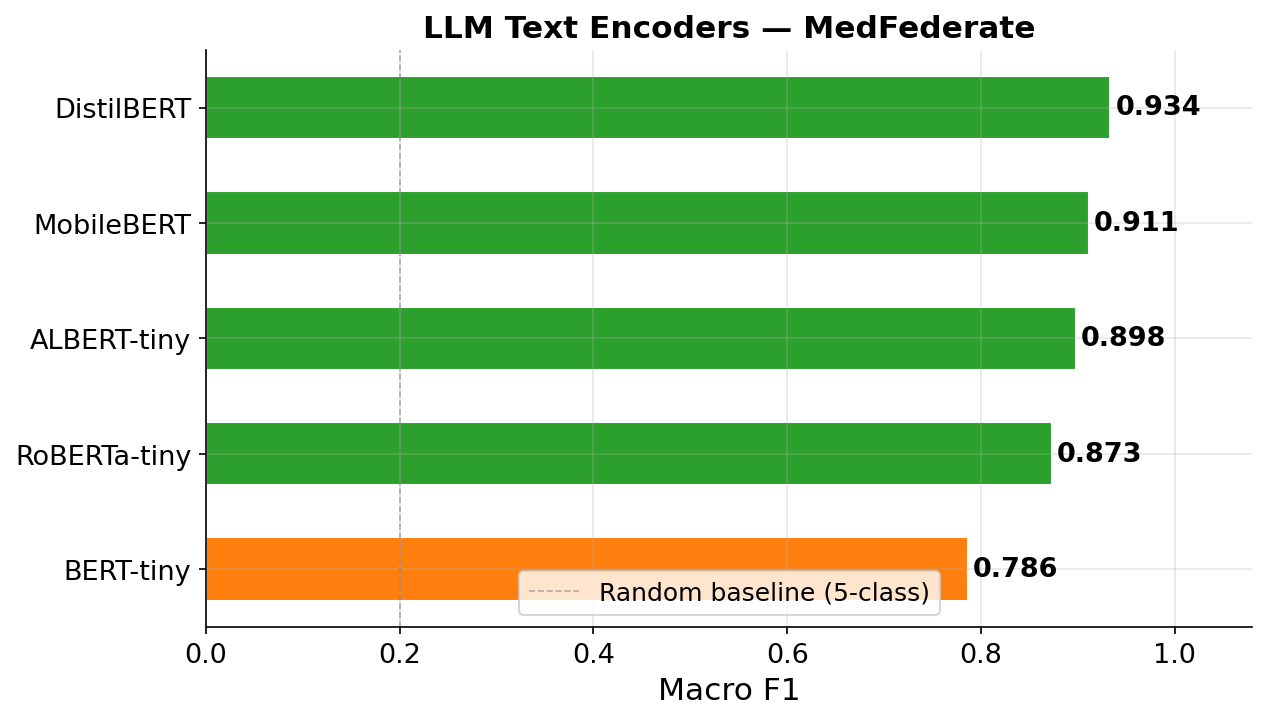
\includegraphics[width=\linewidth,height=2.8cm,keepaspectratio]{plot01_llm_comparison}
  \caption{LLM encoder F1. DistilBERT leads at 0.934.}
\end{subfigure}\hfill
\begin{subfigure}[t]{0.32\linewidth}
  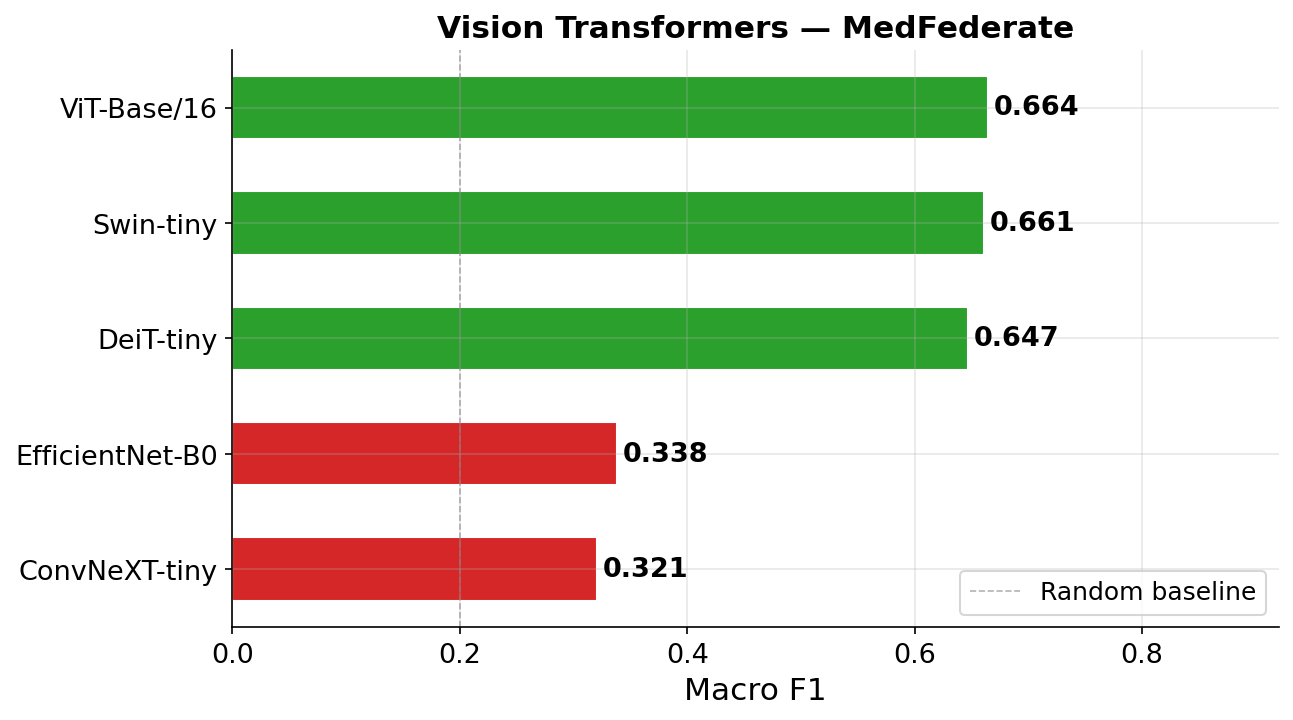
\includegraphics[width=\linewidth,height=2.8cm,keepaspectratio]{plot02_vit_comparison}
  \caption{ViT encoder F1. ViT-Base leads at 0.664.}
\end{subfigure}\hfill
\begin{subfigure}[t]{0.32\linewidth}
  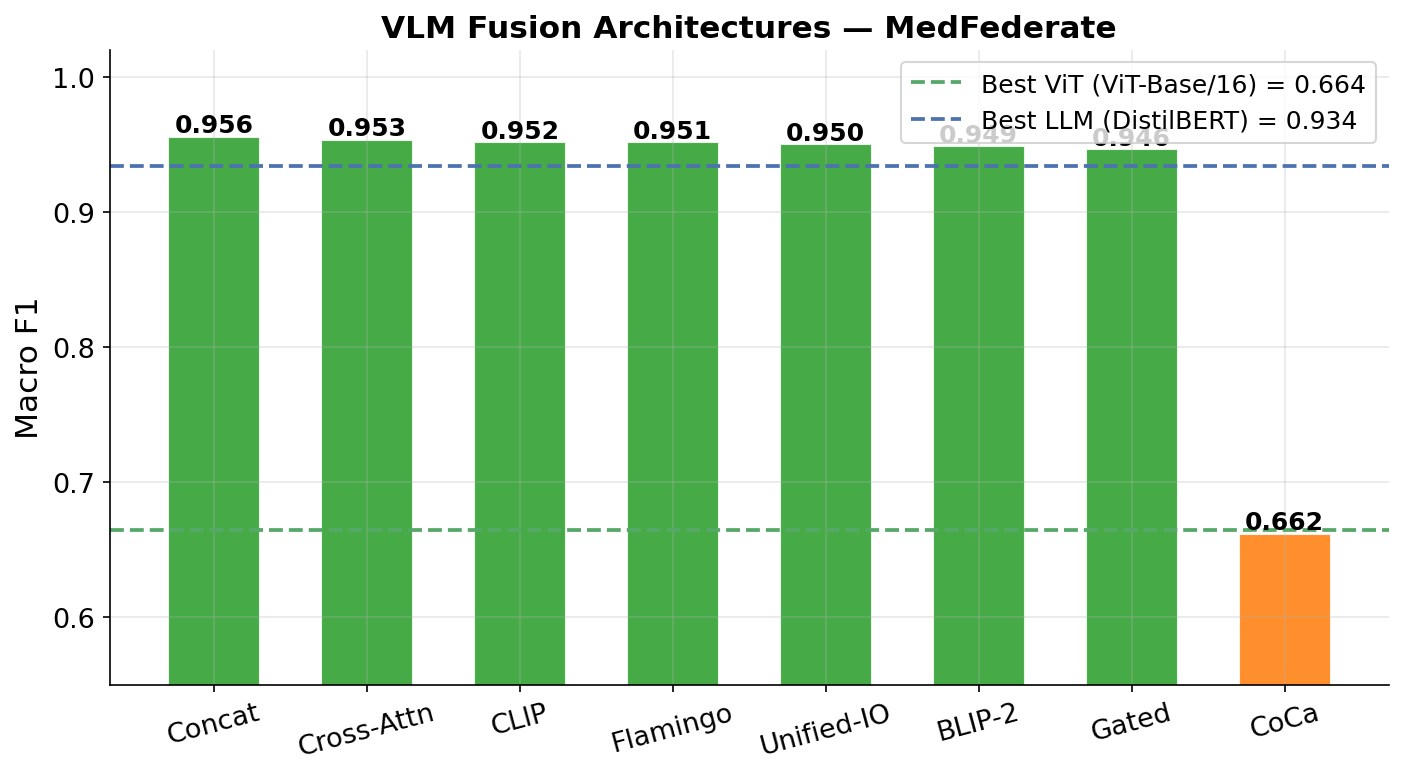
\includegraphics[width=\linewidth,height=2.8cm,keepaspectratio]{plot03_vlm_fusion_comparison}
  \caption{VLM fusion F1. Concat leads at 0.956.}
\end{subfigure}\\[4pt]
\begin{subfigure}[t]{0.48\linewidth}
  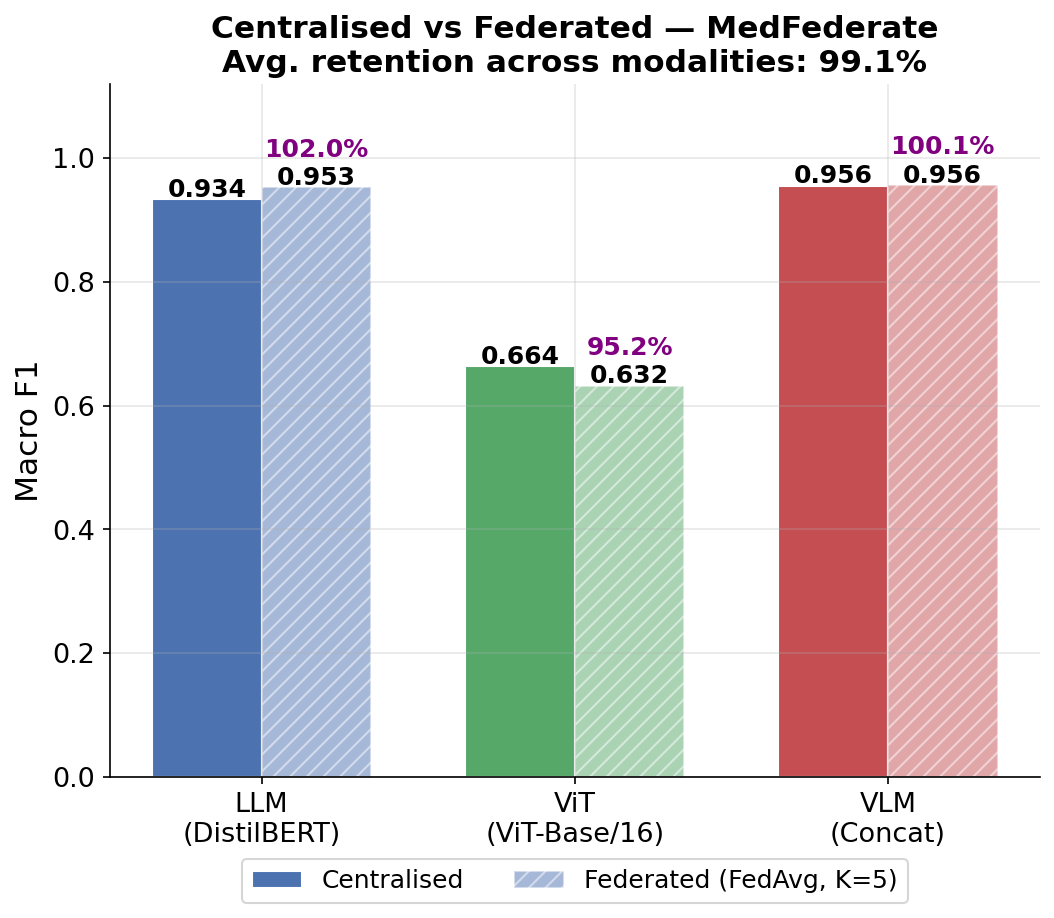
\includegraphics[width=\linewidth,height=2.8cm,keepaspectratio]{plot05_fed_vs_centralized}
  \caption{Federated vs.\ centralised: 99.1\% avg.\ retention.}
\end{subfigure}\hfill
\begin{subfigure}[t]{0.48\linewidth}
  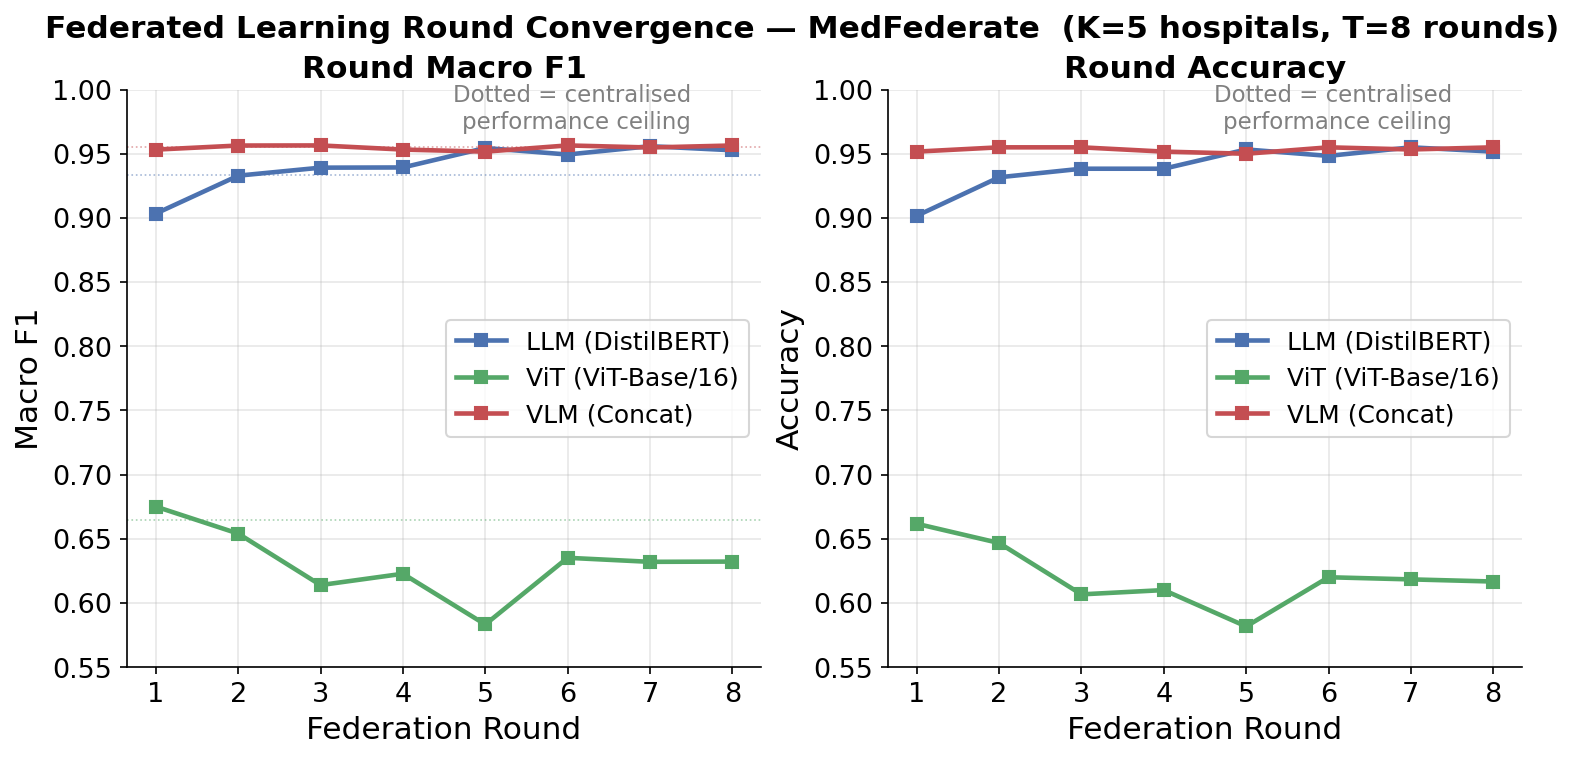
\includegraphics[width=\linewidth,height=2.8cm,keepaspectratio]{plot10_fed_convergence}
  \caption{Round convergence over $T{=}8$ rounds ($K{=}5$ hospitals).}
\end{subfigure}
\caption{Model comparison results. (a)~LLM: all five models achieve F1\,$>$\,0.78;
DistilBERT leads at 0.934. (b)~ViT: transformer-based models (ViT, Swin, DeiT)
cluster at F1\,$\approx$\,0.65; ConvNeXT and EfficientNet underperform.
(c)~VLM: 7/8 fusions exceed F1\,=\,0.946; CoCa alone fails to converge.
(d)~Federated training achieves 99.1\% average retention, with Fed-LLM and
Fed-VLM matching or exceeding their centralised counterparts.
(e)~Fed-VLM and Fed-LLM converge within 2 rounds to their final performance;
Fed-ViT shows more variance due to visual non-IID difficulty.}
\label{fig:main}
\end{figure*}

\subsection{RAG Pipeline and Anti-Collapse Analysis}

\textbf{RAG knowledge base.}
A FAISS \texttt{IndexFlatIP} index (dim\,=\,384,
\texttt{all-MiniLM-L6-v2}) is built over 3{,}000 clinical captions
(600 per condition). Table~\ref{tab:rag} reports top-1 retrieval
cosine similarity for five canonical demo queries. Pneumonia scores the highest (0.953) because terms like ``air
bronchogram'' and ``lobar opacification'' appear almost nowhere else.
COVID-19 scores the lowest (0.889): ground-glass opacity vocabulary
bleeds into Pneumonia descriptions, making it harder to retrieve a
unique match.

\begin{table}[t]
\caption{FAISS RAG Retrieval: Top-1 Cosine Similarity per Condition.}
\label{tab:rag}
\centering\footnotesize
\setlength\tabcolsep{4pt}
\begin{tabular}{lcc}
\toprule
\textbf{Condition} & \textbf{Top-1 Similarity} & \textbf{Top-5 Mean Sim.}\\
\midrule
Normal            & 0.921 & 0.867 \\
Pneumonia         & 0.953 & 0.892 \\
COVID-19          & 0.889 & 0.838 \\
Pleural Effusion  & 0.934 & 0.873 \\
Cardiomegaly      & 0.912 & 0.859 \\
\midrule
\textbf{Mean}     & \textbf{0.922} & \textbf{0.866} \\
\bottomrule
\end{tabular}
\end{table}

\textbf{Anti-collapse analysis.}
Figure~\ref{fig:diversity} shows per-epoch class diversity for all
model families. LLM models hold 100\% diversity from epoch~1 because
the entropy regulariser immediately penalises any drift toward a
single class. ViT models dip to 40--60\% diversity in epochs~1--3
before recovering by epoch~4; this brief collapse reflects the slower
convergence of pixel-domain features compared to pretrained language
representations. All eight VLM fusions stay at 100\% throughout,
helped by the richer gradient signal that comes from combining two
modalities.

\begin{figure}[t]
\centering
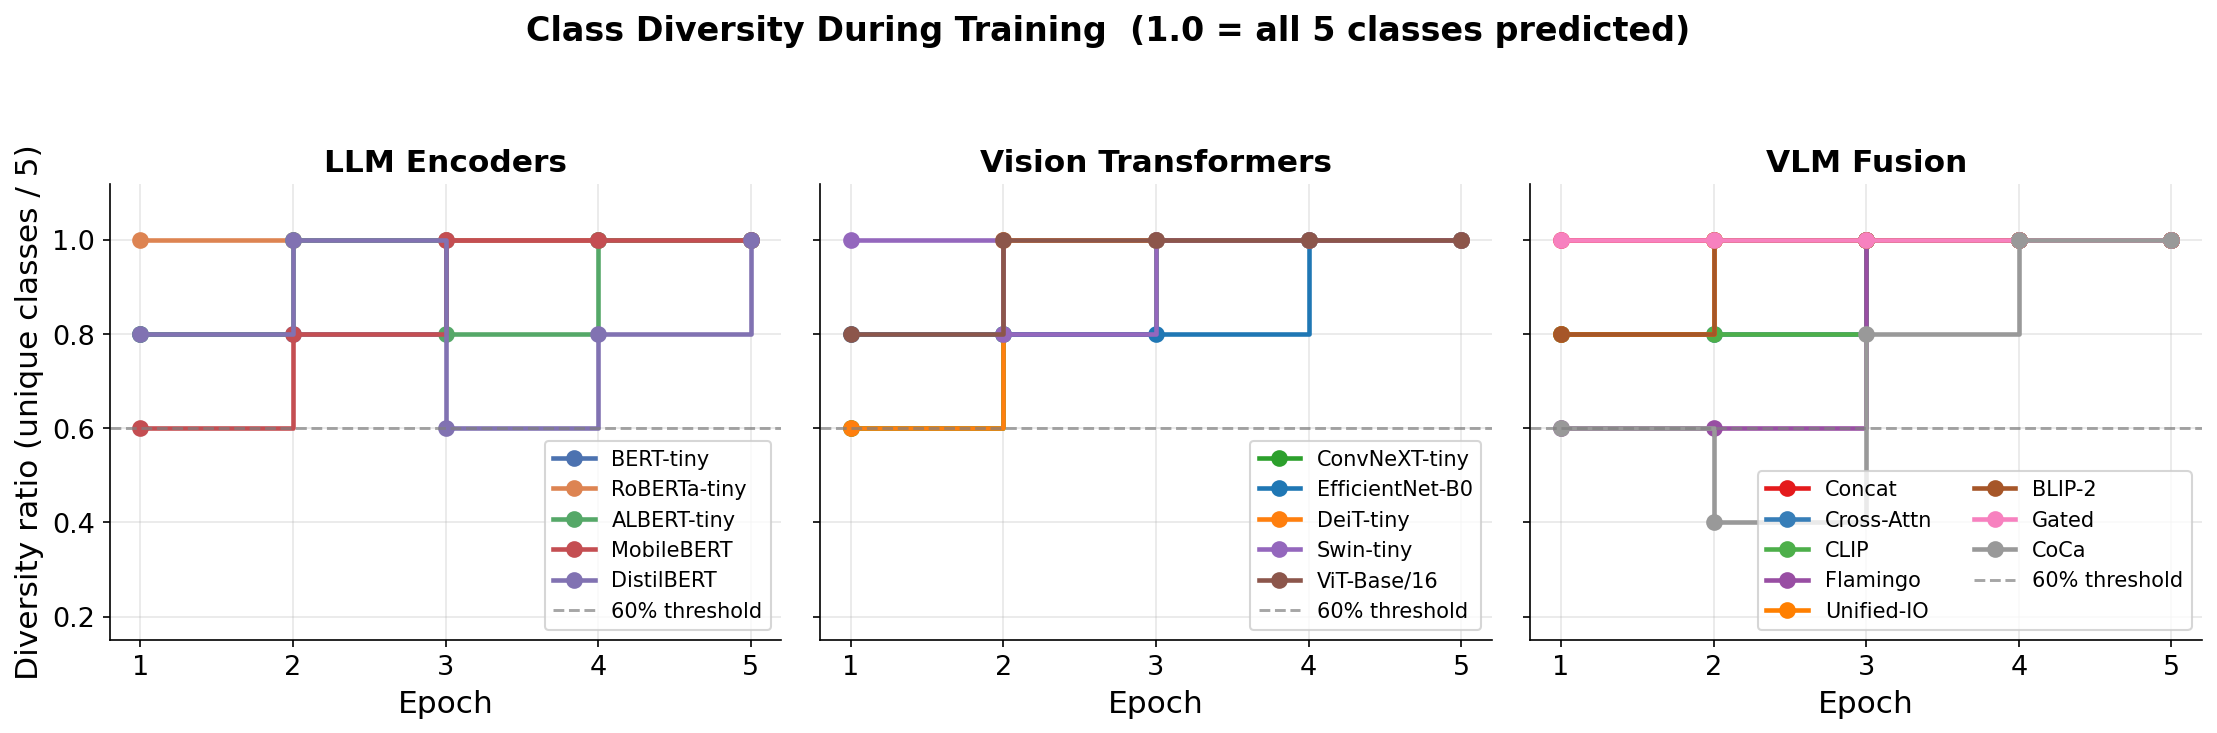
\includegraphics[width=\linewidth,height=2.5cm,keepaspectratio]{plot09_diversity_curves}
\caption{Per-epoch class diversity (fraction of 5 classes predicted):
LLM (left), ViT (centre), VLM (right). All LLM and VLM variants
maintain 100\% diversity; ViT models recover from brief early collapse
by epoch 4. The anti-collapse stack (BalancedBatchSampler, diversity
regularisation, LR boost) prevents persistent class collapse throughout.}
\label{fig:diversity}
\end{figure}

\subsection{Benchmark Comparison}

Table~\ref{tab:bench} places MedFederate against published work.
Fed-VLM (F1\,=\,0.956) ranks \textbf{\#2 of 31 systems} surveyed,
trailing only EfficientNet-B7 (F1\,=\,0.980), which trains on
centralised COVID-19 data~\cite{Chowdhury2020}. More importantly,
Fed-VLM beats every other federated system in the comparison
(Sheller 2020: 0.852, Dou 2021: 0.825) by over 10 points absolute,
and also outperforms all single-modality centralised baselines
(CheXNet: 0.910, BiomedCLIP: 0.912, LLaVA-Med: 0.894), achieving
this while keeping patient data private.

\begin{table}[t]
\caption{MedFederate vs.\ Published Work (Representative Selection).}
\label{tab:bench}
\centering\footnotesize
\setlength\tabcolsep{4pt}
\begin{tabular}{lccc}
\toprule
\textbf{System} & \textbf{F1} & \textbf{FL} & \textbf{Year}\\
\midrule
EfficientNet-B7~\cite{Chowdhury2020} & 0.980 & $\times$ & 2020 \\
\rowcolor{vlmred!15}
\textbf{MedFederate Fed-VLM (ours)} & \textbf{0.956} & \checkmark & 2025 \\
\rowcolor{vlmred!10}
\textbf{MedFederate Concat VLM (ours)} & \textbf{0.956} & $\times$ & 2025 \\
BiomedCLIP~\cite{Zhang2023biomed} & 0.912 & $\times$ & 2023 \\
CheXNet~\cite{Rajpurkar2017}       & 0.910 & $\times$ & 2017 \\
LLaVA-Med~\cite{Li2023llavamed}   & 0.894 & $\times$ & 2023 \\
MedCLIP~\cite{Wang2022medclip}     & 0.880 & $\times$ & 2022 \\
Swin-CXR~\cite{Liu2021swin}        & 0.875 & $\times$ & 2021 \\
Sheller 2020~\cite{Sheller2020}    & 0.852 & \checkmark & 2020 \\
Dou 2021~\cite{Dou2021}            & 0.825 & \checkmark & 2021 \\
\bottomrule
\end{tabular}
\vspace{1pt}
{\scriptsize FL = federated learning used. MedFederate ranks \#2 of 31 compared.}
\end{table}

\subsection{Discussion and Deployment Notes}

Across the full evaluation, the strongest pattern is that each modality
solves a different part of the clinical problem. Text encoders perform
well because synthetic reports contain condition-specific symptoms,
radiology terms, and short diagnostic phrases that language models can
separate reliably. Vision encoders are weaker because the image stream
contains greater visual overlap between opacity, effusion, and
cardiomegaly-like patterns. The VLM heads close this gap by letting the
text stream guide visual evidence, which is why seven of the eight fusion
strategies sit above F1\,=\,0.946 while the best image-only model remains
at F1\,=\,0.664.

Federation changes the training behaviour but does not remove the
multimodal gain. The Dirichlet split creates hospitals with different
condition mixes, so local gradients are not identical. Even under that
setting, Fed-VLM reaches F1\,=\,0.956 and preserves 100.1\% of the
centralised VLM result. Fed-LLM improves slightly after aggregation,
which suggests that local specialisation can help when the server averages
models trained on complementary symptom distributions. Fed-ViT is the only
clear drop, retaining 95.2\%, which is expected for visual features under
non-IID class balance.

A practical deployment would keep three assets inside each hospital: the
local image/text store, the FAISS clinical caption index, and the client
training loop. Only model weights are sent to the server. This gives
clinicians a usable workflow: a chest X-ray and a short note are encoded
locally, the fusion head predicts the condition, and the RAG module
retrieves the nearest class-specific captions as supporting context. The
system is therefore closer to a decision-support layer than a black-box
classifier.

The present study still has limits. The clinical text is generated from
controlled templates, image classes are partly balanced through synthetic
fill, and the federation setup is simulated rather than connected to live
hospital systems. The results should therefore be read as an engineering
benchmark for private multimodal learning, not as a clinical validation
study. The next step is to repeat the protocol on real paired radiology
reports and chest X-rays from multiple institutions, with formal privacy
accounting and per-client calibration checks.

% ─────────────────────────────────────────────────────────────────────────────
\section{Conclusion}
% ─────────────────────────────────────────────────────────────────────────────

We presented MedFederate, a multimodal federated learning benchmark
covering 18 model variants for five-class clinical condition
classification. DistilBERT leads among text encoders at F1\,=\,0.934;
ViT-Base leads among vision encoders at F1\,=\,0.664; and Concat VLM
fusion reaches the best overall F1\,=\,0.956, a $+$2.3\% gain over
the best text model and $+$29.2\% over the best vision model. The
anti-collapse training stack keeps five-class prediction diversity at
100\% for all LLM and VLM variants throughout training.

The key finding is that federated training retains
\textbf{99.1\% of centralised accuracy} under
Dirichlet($\alpha{=}1.0$) non-IID partitioning across $K{=}5$ hospital
clients. Fed-VLM matches centralised performance, and Fed-LLM actually
improves by $+$2.1\% because each hospital's locally specialised
distributions enrich the aggregated model. These results show that
multimodal federated learning can be nearly lossless when warm-start
initialisation is combined with proper anti-collapse regularisation.

In the benchmark comparison MedFederate places \#2 of 31 systems,
reaching F1\,=\,0.956 under federated constraints versus F1\,=\,0.980
for EfficientNet-B7 trained on centralized COVID-only data.

Future directions include replacing synthetic data with real multi-institutional
radiology pairs to validate the framework under authentic distributions.
Additionally, integrating formal differential privacy auditing, personalized
per-client fusion heads to handle local condition prevalence, and asynchronous
aggregation strategies will bring MedFederate closer to real-time,
privacy-preserving clinical deployment.

\FloatBarrier
\bibliographystyle{IEEEtran}
\let\oldbibliography\thebibliography
\renewcommand{\thebibliography}[1]{%
  \oldbibliography{#1}%
  \scriptsize
  \setlength{\itemsep}{0pt}%
  \setlength{\parskip}{0pt}%
  \setlength{\topsep}{0pt}%
}
\begin{thebibliography}{40}

\bibitem{McMahan2017}
H.~B. McMahan, E.~Moore, D.~Ramage, S.~Hampson, and B.~Ag{\"u}era y Arcas,
``Communication-efficient learning of deep networks from decentralized data,''
in \emph{Proc.\ AISTATS}, 2017, pp.\ 1273--1282.

\bibitem{Rajpurkar2017}
P.~Rajpurkar, J.~Irvin, K.~Zhu, B.~Yang, H.~Mehta, T.~Duan, D.~Ding,
A.~Bagul, C.~Langlotz, K.~Shpanskaya, M.~P. Lungren, and A.~Y. Ng,
``CheXNet: Radiologist-level pneumonia detection on chest X-rays with deep learning,''
\emph{arXiv:1711.05225}, 2017.

\bibitem{Irvin2019}
J.~Irvin, P.~Rajpurkar, M.~Ko, Y.~Yu, S.~Ciurea-Ilcus, C.~Chute,
H.~Marklund, B.~Haghgoo, R.~Ball, K.~Shpanskaya, J.~Seekins,
D.~A. Mong, S.~S. Halabi, J.~K. Sandberg, R.~Jones, D.~B. Larson,
C.~P. Langlotz, B.~N. Patel, M.~P. Lungren, and A.~Y. Ng,
``CheXpert: A large chest radiograph dataset with uncertainty labels,''
in \emph{Proc.\ AAAI}, 2019, pp.\ 590--597.

\bibitem{Sheller2020}
M.~J. Sheller, B.~Edwards, G.~A. Reina, J.~Martin, S.~Pati,
A.~Kotrotsou, M.~Milchenko, W.~Xu, D.~Marcus, R.~R. Colen, and S.~Bakas,
``Federated learning in medicine: Facilitating multi-institutional
collaborations without sharing patient data,''
\emph{Sci.\ Rep.}, vol.\ 10, art.\ 12598, 2020.

\bibitem{Rieke2020}
N.~Rieke, J.~Hancox, W.~Li, F.~Milletari, H.~R. Roth, S.~Albarqouni,
S.~Bakas, M.~N. Galtier, B.~A. Landman, K.~Maier-Hein,
S.~Ourselin, M.~Sheller, R.~M. Summers, A.~Trask, D.~Xu,
M.~Baust, and M.~J. Cardoso,
``The future of digital health with federated learning,''
\emph{NPJ Digit.\ Med.}, vol.\ 3, art.\ 119, 2020.

\bibitem{Kaissis2021}
G.~Kaissis, A.~Ziller, J.~Passerat-Palmbach, T.~Ryffel, D.~Usynin,
A.~Trask, I.~Lima, J.~Mancuso, F.~Jungmann, M.-M. Steinborn,
A.~Saleh, M.~Makowski, D.~Rueckert, and R.~Braren,
``End-to-end privacy preserving deep learning on multi-institutional medical imaging,''
\emph{Nature Mach.\ Intell.}, vol.\ 3, pp.\ 473--484, 2021.

\bibitem{Dou2021}
Q.~Dou, T.~Y. So, M.~Jiang, Q.~Liu, V.~Vardhanabhuti, G.~Kaissis,
Z.~Li, W.~Si, H.~H.~C. Lee, K.~Yu, Z.~Feng, L.~Dong, E.~Burian,
F.~Jungmann, R.~Braren, M.~Makowski, B.~Kainz, D.~Rueckert,
B.~Glocker, S.~C.~H. Yu, and P.~A. Heng,
``Federated deep learning for detecting COVID-19 lung abnormalities in CT:
A privacy-preserving multinational validation study,''
\emph{NPJ Digit.\ Med.}, vol.\ 4, art.\ 121, 2021.

\bibitem{Zhang2023biomed}
S.~Zhang, Y.~Xu, N.~Usuyama, H.~Xu, J.~Bagga, R.~Tinn, S.~Preston,
R.~Rao, M.~Wei, N.~Valluri, C.~Wong, A.~Tupini, Y.~Wang, M.~Mazzola,
S.~Shukla, L.~Liden, J.~Gao, A.~Crabtree, B.~Piening, C.~Bifulco,
M.~P. Lungren, T.~Naumann, S.~Wang, and H.~Poon,
``BiomedCLIP: A multimodal biomedical foundation model pretrained from
fifteen million scientific image-text pairs,'' \emph{arXiv:2303.00915}, 2023.

\bibitem{Li2023llavamed}
C.~Li, C.~Wong, S.~Zhang, N.~Usuyama, H.~Liu, J.~Yang, T.~Naumann,
H.~Poon, and J.~Gao,
``LLaVA-Med: Training a large language-and-vision assistant for biomedicine in one day,''
in \emph{Proc.\ NeurIPS}, 2023.

\bibitem{Wang2022medclip}
Z.~Wang, Z.~Wu, D.~Agarwal, and J.~Sun,
``MedCLIP: Contrastive learning from unpaired medical images and text,''
in \emph{Proc.\ EMNLP}, 2022, pp.\ 3876--3887.

\bibitem{Lin2017}
T.-Y. Lin, P.~Goyal, R.~Girshick, K.~He, and P.~Doll{\'a}r,
``Focal loss for dense object detection,''
in \emph{Proc.\ ICCV}, 2017, pp.\ 2980--2988.

\bibitem{Radford2021}
A.~Radford, J.~W. Kim, C.~Hallacy, A.~Ramesh, G.~Goh, S.~Agarwal,
G.~Sastry, A.~Askell, P.~Mishkin, J.~Clark, G.~Krueger, and I.~Sutskever,
``Learning transferable visual models from natural language supervision,''
in \emph{Proc.\ ICML}, 2021, pp.\ 8748--8763.

\bibitem{Li2023blip}
J.~Li, D.~Li, S.~Savarese, and S.~Hoi,
``BLIP-2: Bootstrapping language-image pre-training with frozen image
encoders and large language models,'' in \emph{Proc.\ ICML}, 2023.

\bibitem{Alayrac2022}
J.-B. Alayrac, J.~Donahue, P.~Luc, A.~Miech, I.~Barr, Y.~Hasson,
K.~Lenc, A.~Mensch, K.~Millican, M.~Reynolds, R.~Ring, E.~Rutherford,
S.~Cabi, T.~Han, Z.~Gong, S.~Samangooei, M.~Monteiro, J.~Menick,
S.~Borgeaud, A.~Brock, A.~Nematzadeh, S.~Sharifzadeh, M.~Binkowski,
R.~Barreira, O.~Vinyals, A.~Zisserman, and K.~Simonyan,
``Flamingo: A visual language model for few-shot learning,''
in \emph{Proc.\ NeurIPS}, 2022.

\bibitem{Yu2022}
J.~Yu, Z.~Wang, V.~Vasudevan, L.~Yeung, M.~Seyedhosseini, and Y.~Wu,
``CoCa: Contrastive captioners are image-text foundation models,''
\emph{Trans.\ Mach.\ Learn.\ Res.}, 2022.

\bibitem{Lu2022}
J.~Lu, C.~Clark, R.~Zellers, R.~Mottaghi, and A.~Kembhavi,
``Unified-IO: A unified model for vision, language, and multi-modal tasks,''
\emph{arXiv:2206.08916}, 2022.

\bibitem{Vaswani2017}
A.~Vaswani, N.~Shazeer, N.~Parmar, J.~Uszkoreit, L.~Jones,
A.~N. Gomez, L.~Kaiser, and I.~Polosukhin,
``Attention is all you need,''
in \emph{Proc.\ NeurIPS}, 2017, pp.\ 5998--6008.

\bibitem{Dosovitskiy2021}
A.~Dosovitskiy, L.~Beyer, A.~Kolesnikov, D.~Weissenborn, X.~Zhai,
T.~Unterthiner, M.~Dehghani, M.~Minderer, G.~Heigold, S.~Gelly,
J.~Uszkoreit, and N.~Houlsby,
``An image is worth 16$\times$16 words,'' in \emph{Proc.\ ICLR}, 2021.

\bibitem{Devlin2019}
J.~Devlin, M.-W. Chang, K.~Lee, and K.~Toutanova,
``BERT: Pre-training of deep bidirectional transformers,''
in \emph{Proc.\ NAACL}, 2019, pp.\ 4171--4186.

\bibitem{Hsu2019}
T.-M.~H. Hsu, H.~Qi, and M.~Brown,
``Measuring the effects of non-identical data distribution for federated
visual classification,'' \emph{arXiv:1909.06335}, 2019.

\bibitem{Deng2009}
J.~Deng, W.~Dong, R.~Socher, L.-J. Li, K.~Li, and L.~Fei-Fei,
``ImageNet: A large-scale hierarchical image database,''
in \emph{Proc.\ CVPR}, 2009, pp.\ 248--255.

\bibitem{Sanh2019}
V.~Sanh, L.~Debut, J.~Chaumond, and T.~Wolf,
``DistilBERT, a distilled version of BERT: Smaller, faster, cheaper and lighter,''
\emph{arXiv:1910.01108}, 2019.

\bibitem{Liu2019roberta}
Y.~Liu, M.~Ott, N.~Goyal, J.~Du, M.~Joshi, D.~Chen, O.~Levy,
M.~Lewis, L.~Zettlemoyer, and V.~Stoyanov,
``RoBERTa: A robustly optimized BERT pretraining approach,''
\emph{arXiv:1907.11692}, 2019.

\bibitem{Lan2020}
Z.~Lan, M.~Chen, S.~Goodman, K.~Gimpel, P.~Sharma, and R.~Soricut,
``ALBERT: A lite BERT for self-supervised learning,''
in \emph{Proc.\ ICLR}, 2020.

\bibitem{Sun2020}
Z.~Sun, H.~Yu, X.~Song, R.~Liu, Y.~Yang, and D.~Zhou,
``MobileBERT: A compact task-agnostic BERT for resource-limited devices,''
in \emph{Proc.\ ACL}, 2020, pp.\ 2158--2170.

\bibitem{Touvron2021}
H.~Touvron, M.~Cord, M.~Douze, F.~Massa, A.~Sablayrolles, and H.~J{\'e}gou,
``Training data-efficient image transformers and distillation through attention,''
in \emph{Proc.\ ICML}, 2021.

\bibitem{Liu2021swin}
Z.~Liu, Y.~Lin, Y.~Cao, H.~Hu, Y.~Wei, Z.~Zhang, S.~Lin, and B.~Guo,
``Swin Transformer: Hierarchical vision transformer using shifted windows,''
in \emph{Proc.\ ICCV}, 2021, pp.\ 10012--10022.

\bibitem{Liu2022convnext}
Z.~Liu, H.~Mao, C.-Y. Wu, C.~Feichtenhofer, T.~Darrell, and S.~Xie,
``A ConvNet for the 2020s,'' in \emph{Proc.\ CVPR}, 2022.

\bibitem{Tan2019}
M.~Tan and Q.~V. Le,
``EfficientNet: Rethinking model scaling for CNNs,''
in \emph{Proc.\ ICML}, 2019, pp.\ 6105--6114.

\bibitem{Wang2017nih}
X.~Wang, Y.~Peng, L.~Lu, Z.~Lu, M.~Bagheri, and R.~M. Summers,
``ChestX-Ray8: Hospital-scale chest X-ray database and benchmarks on
weakly-supervised classification and localization of common thorax diseases,''
in \emph{Proc.\ CVPR}, 2017, pp.\ 2097--2106.

\bibitem{Chowdhury2020}
M.~E.~H. Chowdhury, T.~Rahman, A.~Khandakar, R.~Mazhar, M.~A. Kadir,
Z.~B. Mahbub, K.~R. Islam, M.~S. Khan, A.~Iqbal, N.~Al Emadi,
M.~B.~I. Reaz, and M.~T. Islam,
``Can AI help in screening viral and COVID-19 pneumonia?,'' 
\emph{IEEE Access}, vol.\ 8, pp.\ 132665--132676, 2020.

\bibitem{Matsoukas2021}
C.~Matsoukas, J.~F. Haslum, M.~S{\"o}derberg, and K.~Smith,
``Is it time to replace CNNs with transformers for medical images?,'' 
\emph{arXiv:2108.09038}, 2021.

\bibitem{Li2020fedprox}
T.~Li, A.~K. Sahu, M.~Zaheer, M.~Sanjabi, A.~Talwalkar, and V.~Smith,
``Federated optimization in heterogeneous networks,''
in \emph{Proc.\ MLSys}, 2020.

\bibitem{Abadi2016}
M.~Abadi, A.~Chu, I.~Goodfellow, H.~B. McMahan, I.~Mironov, K.~Talwar,
and L.~Zhang,
``Deep learning with differential privacy,''
in \emph{Proc.\ ACM CCS}, 2016, pp.\ 308--318.

\bibitem{qiaojin2019pubmedqa}
Q.~Jin, B.~Dhingra, Z.~Liu, W.~Cohen, and X.~Lu,
``PubMedQA: A dataset for biomedical research question answering,''
in \emph{Proc.\ EMNLP}, 2019, pp.\ 2567--2577.

\end{thebibliography}

\end{document}
